\section{Evaluation}
\label{sec:evaluation}

% TODO: Setting.  Computer resources (CPU, RAM, OS).

\subsection{Setup}

We have evaluated our implementation in an environment consisting on two
computers located in the same gigabit ethernet network.  We run the Broker,
Third Party and one Subscriber on the first computer, and all the Publishers in
the second computer.  We perform all the analysis on the performance of several
operations in the Broker and Third Party, which run together in a computer
running Linux with an Intel Core i7-6600U CPU with 16GB of RAM.  In order to
avoid isolate the performance influence of the Broker and the Third Party, we
have serialized the garbling and evaluation of the garbled circuit operations,
mimicking the situation in which the Broker and Third Party are run on
different servers.

\subsection{Microbenchmarks}

We have selected 5 numerical operations of varying complexity (\emph{summation,
multiplicatory, mean, variance, minimum}) to evaluate the cost of the different
parts of our implementation.  We securely evaluate these functions over the
values (encoded as 32 bit fixed point numbers) received from a variable number
of Publishers.

% TODO: Indicate the number of experiments per value

% Plots
\begin{figure*}
    \centering
    \begin{subfigure}[b]{0.32\textwidth}
        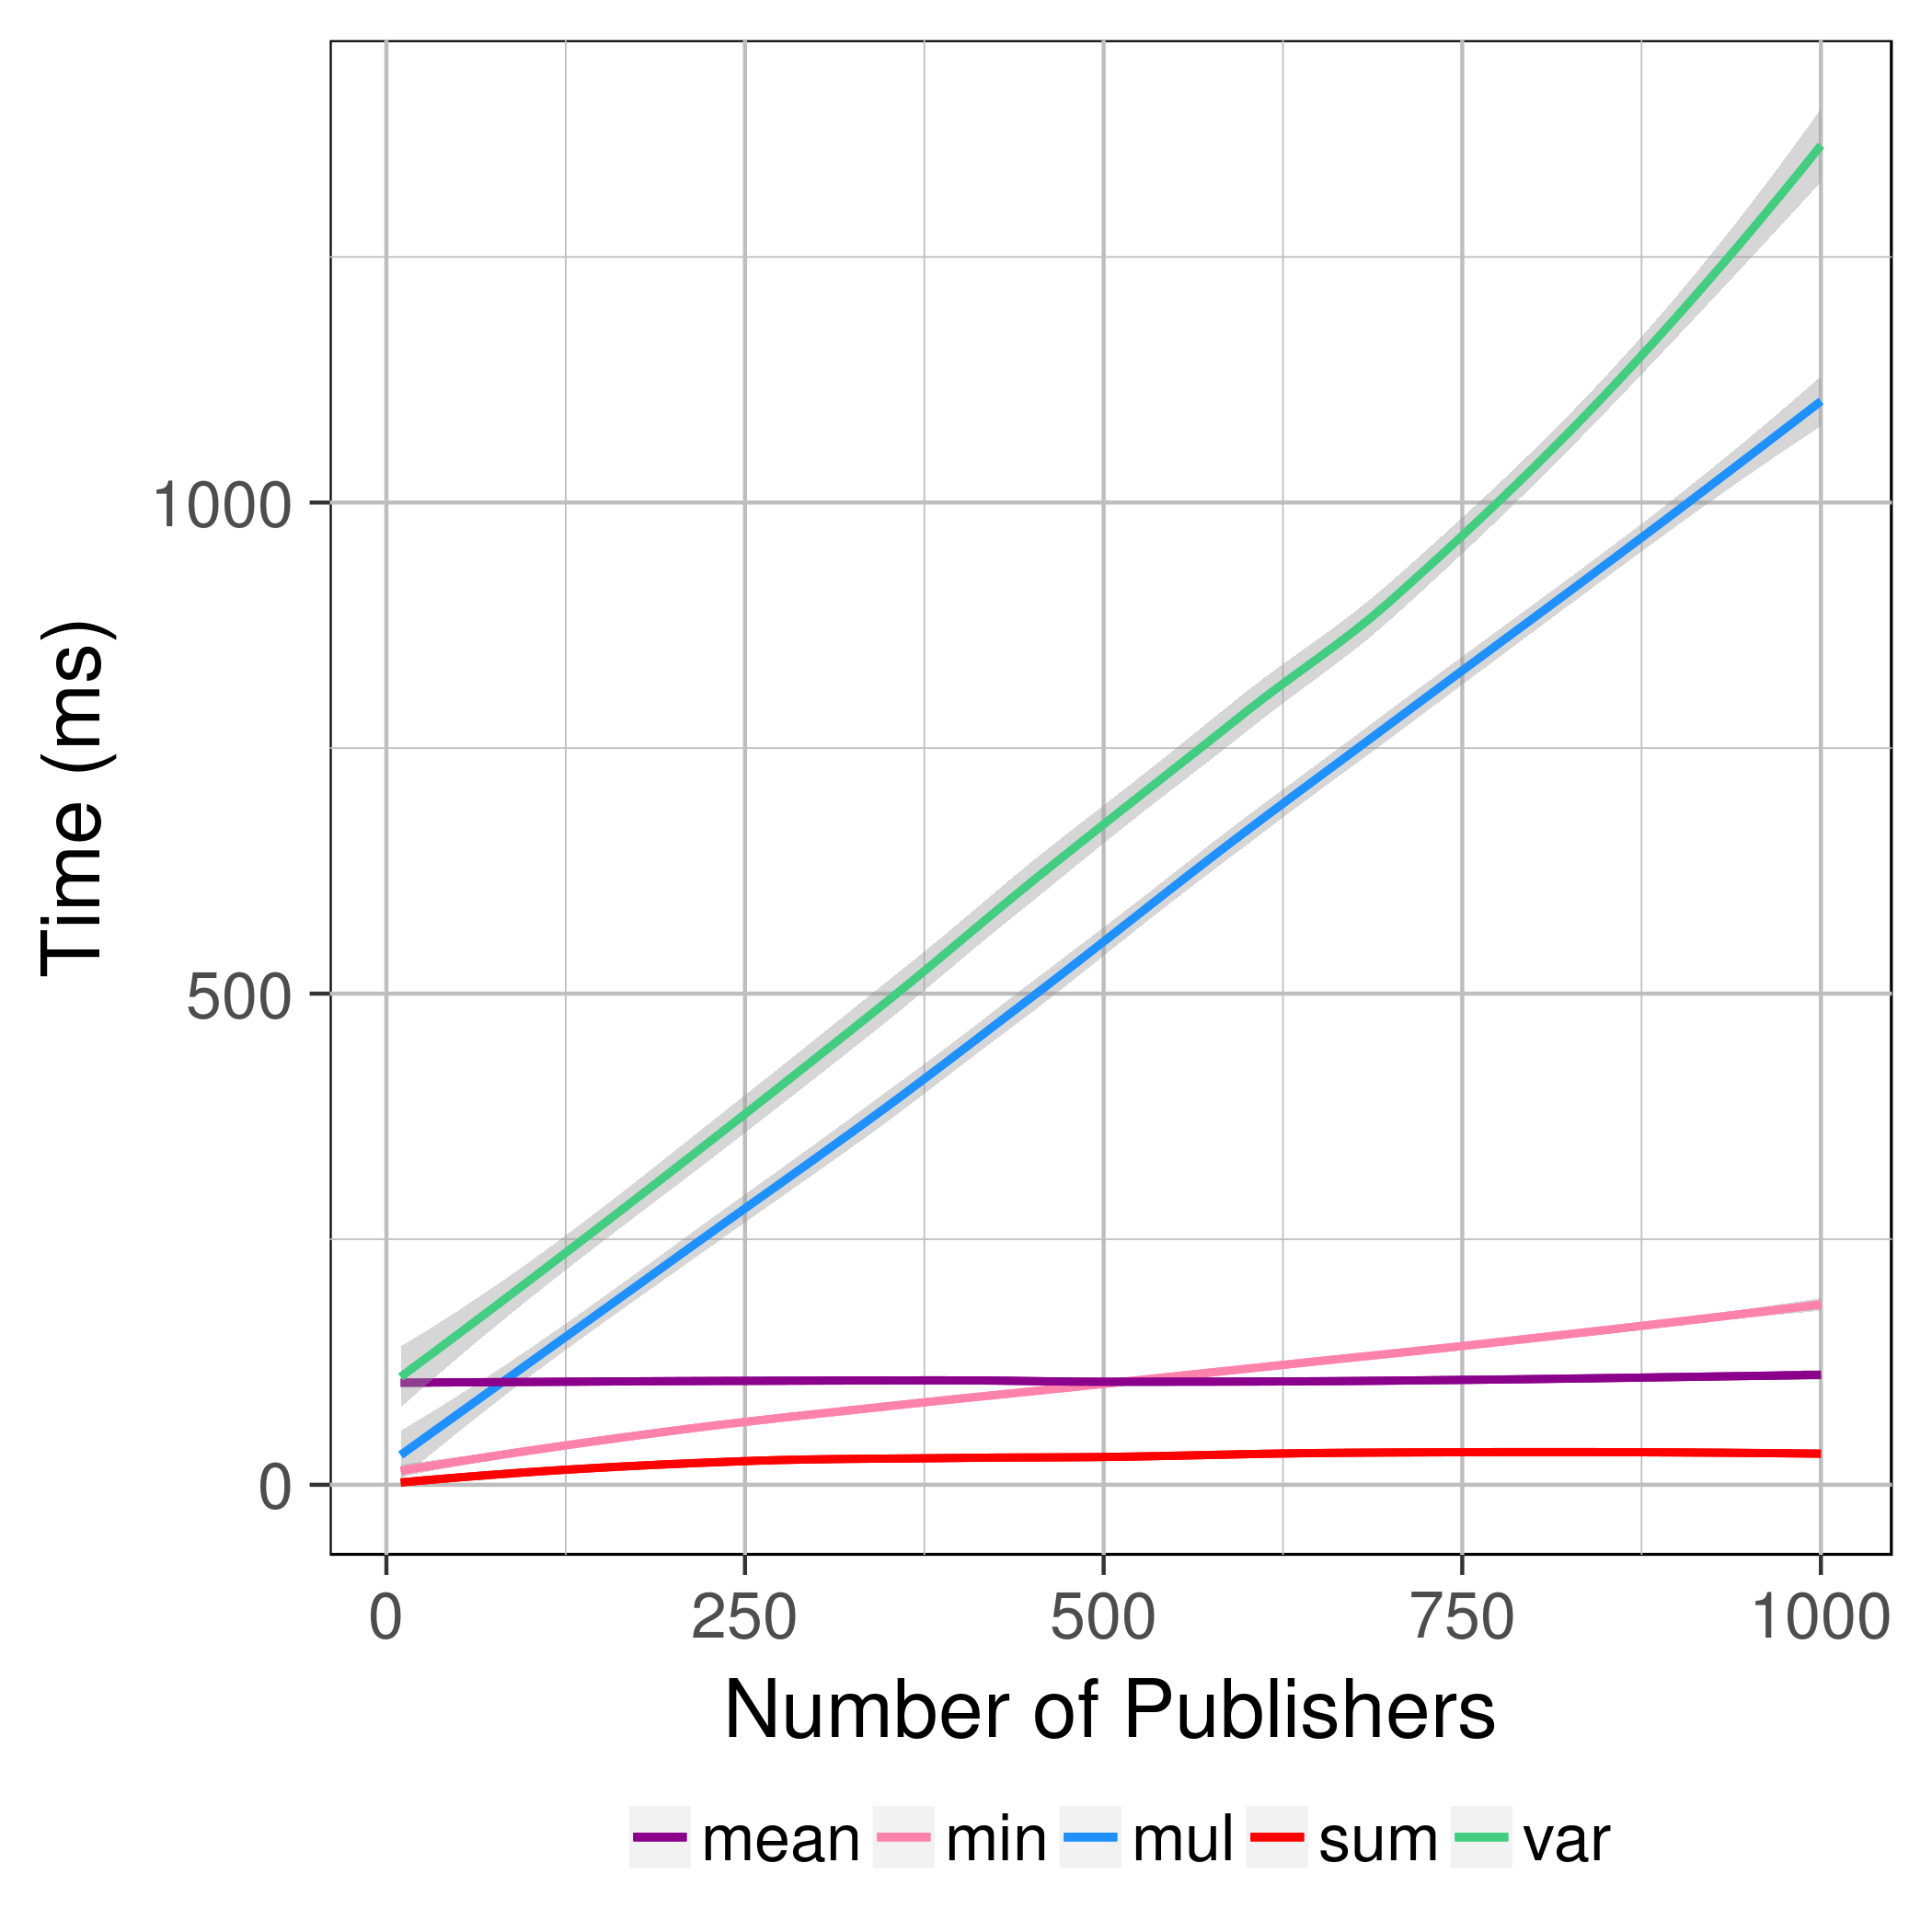
\includegraphics[width=\textwidth]{plots/garble.png}
        \caption{Garble}
        \label{fig:micro-garble-time}
    \end{subfigure}
    ~ %add desired spacing between images, e. g. ~, \quad, \qquad, \hfill etc.
    \begin{subfigure}[b]{0.32\textwidth}
        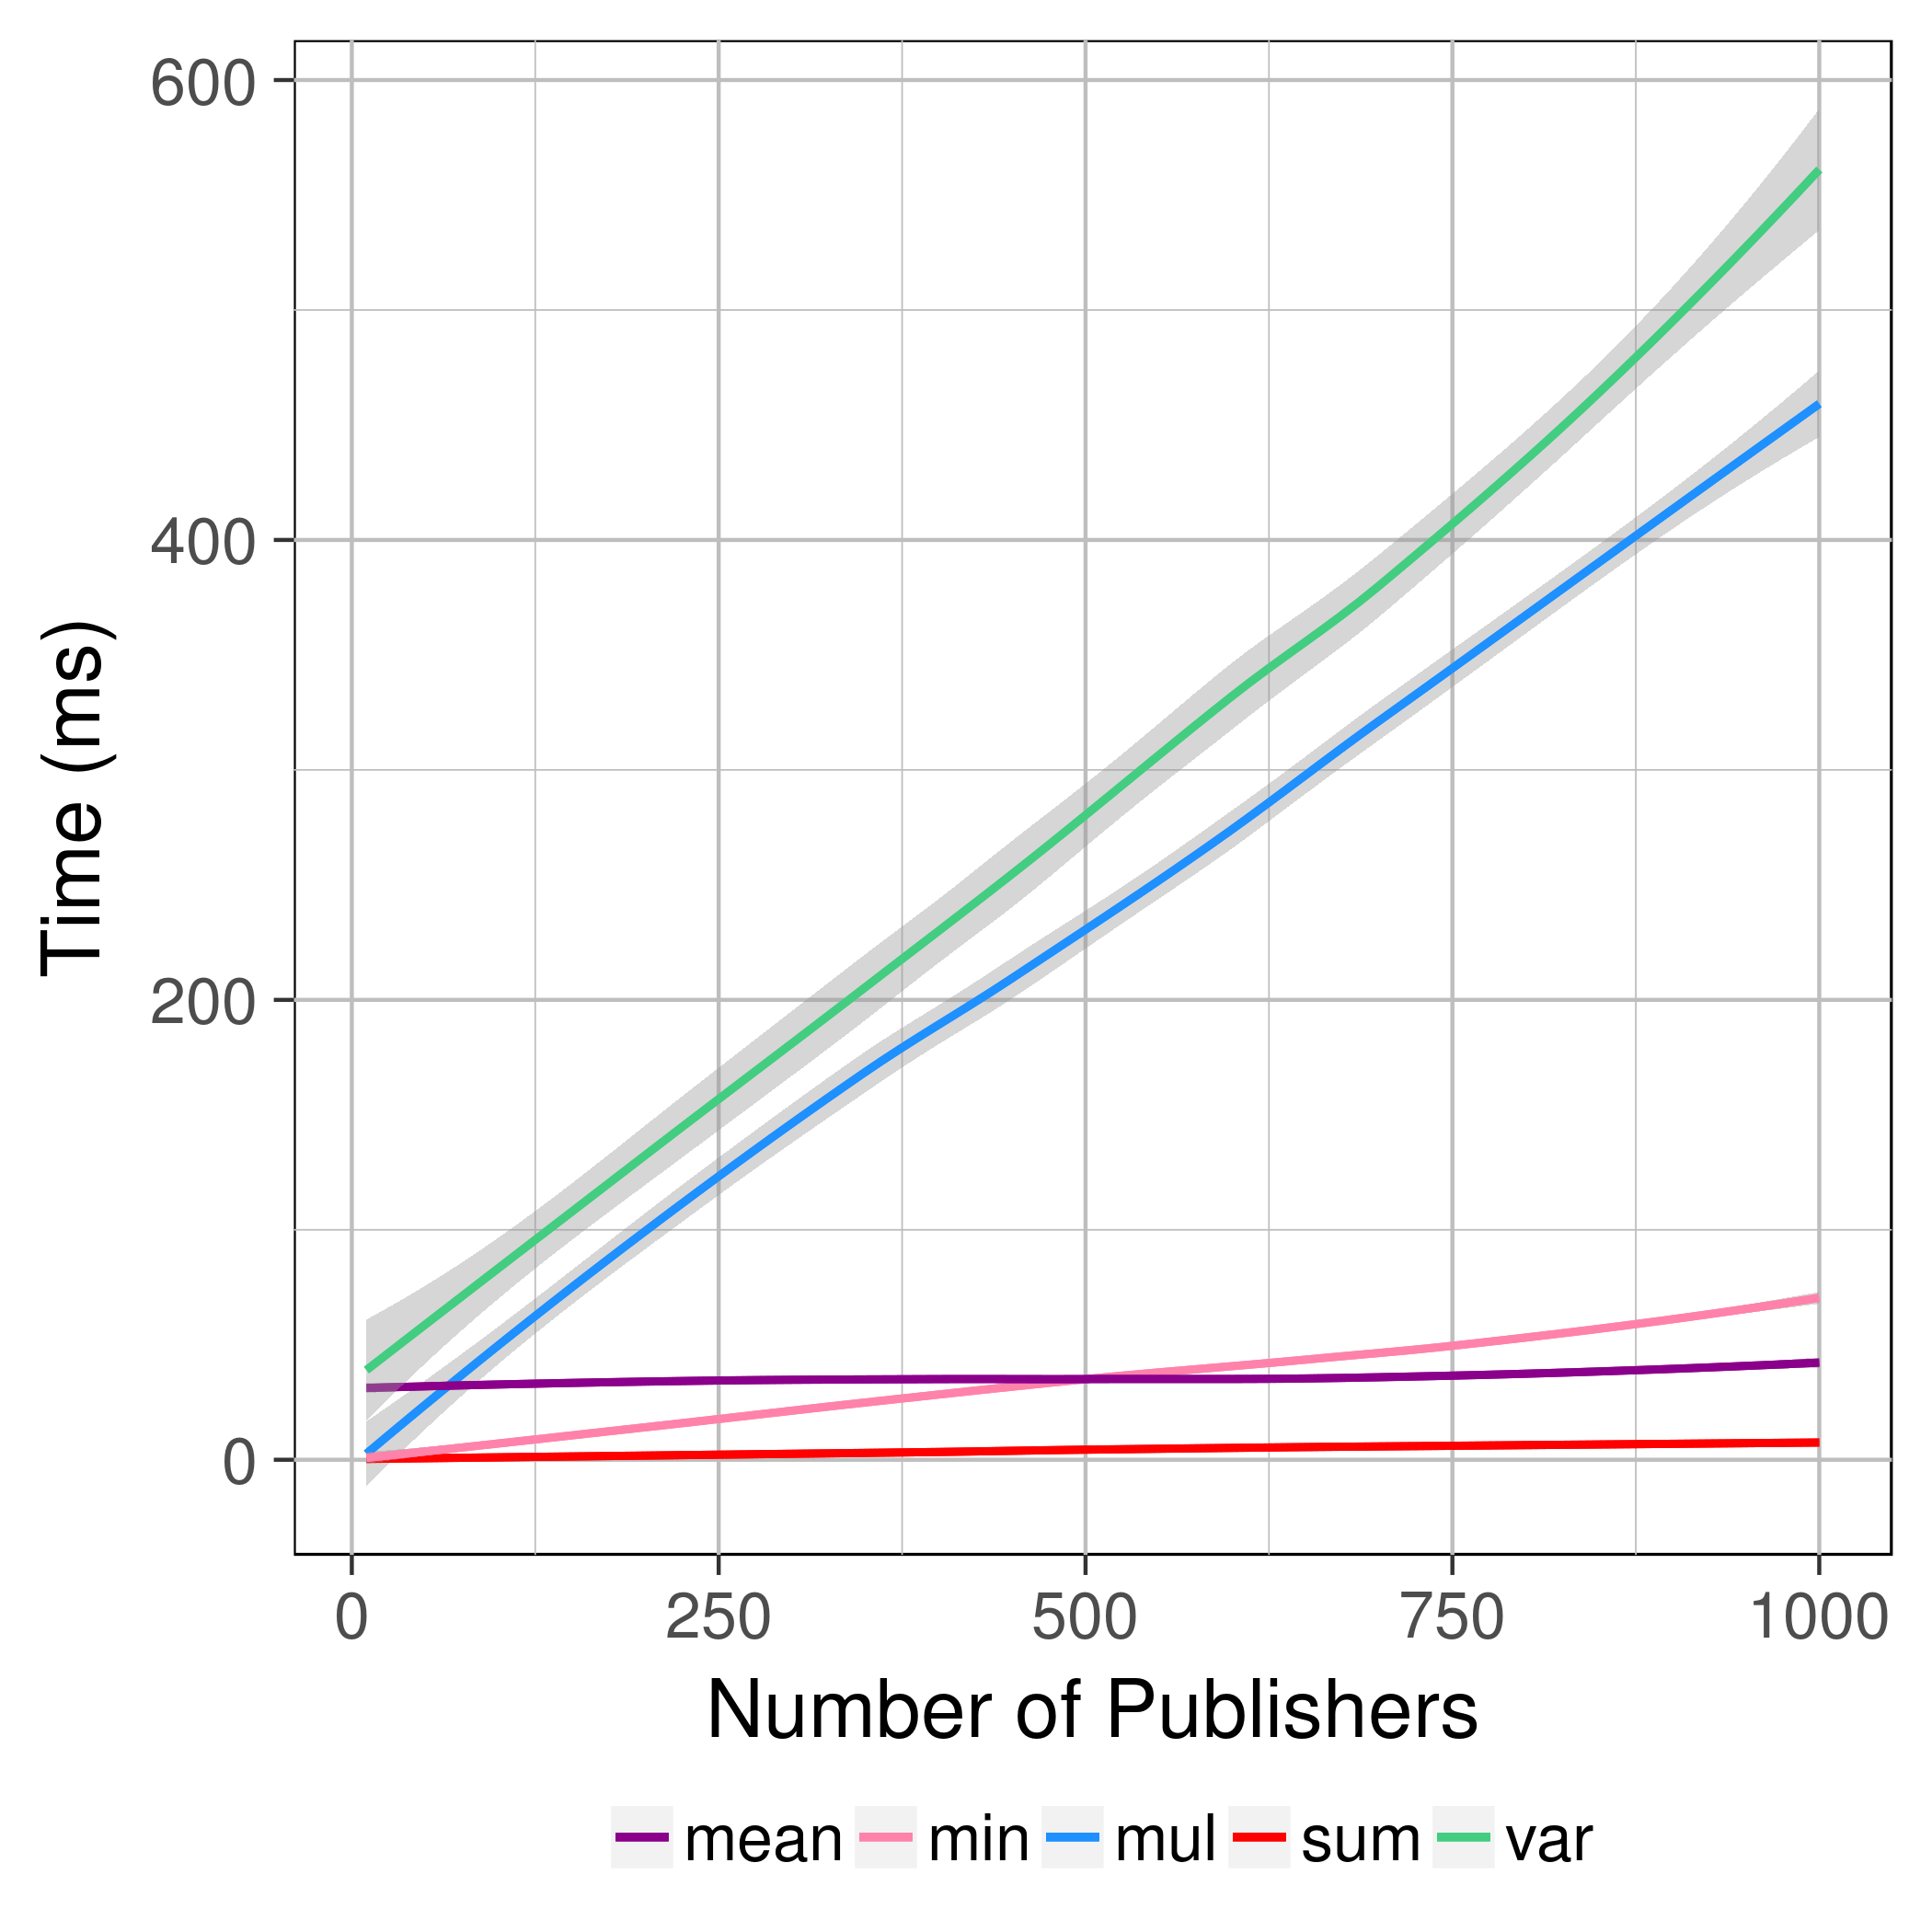
\includegraphics[width=\textwidth]{plots/eval.png}
        \caption{Evaluate}
        \label{fig:micro-eval-time}
    \end{subfigure}
    ~ %add desired spacing between images, e. g. ~, \quad, \qquad, \hfill etc.
    \begin{subfigure}[b]{0.32\textwidth}
        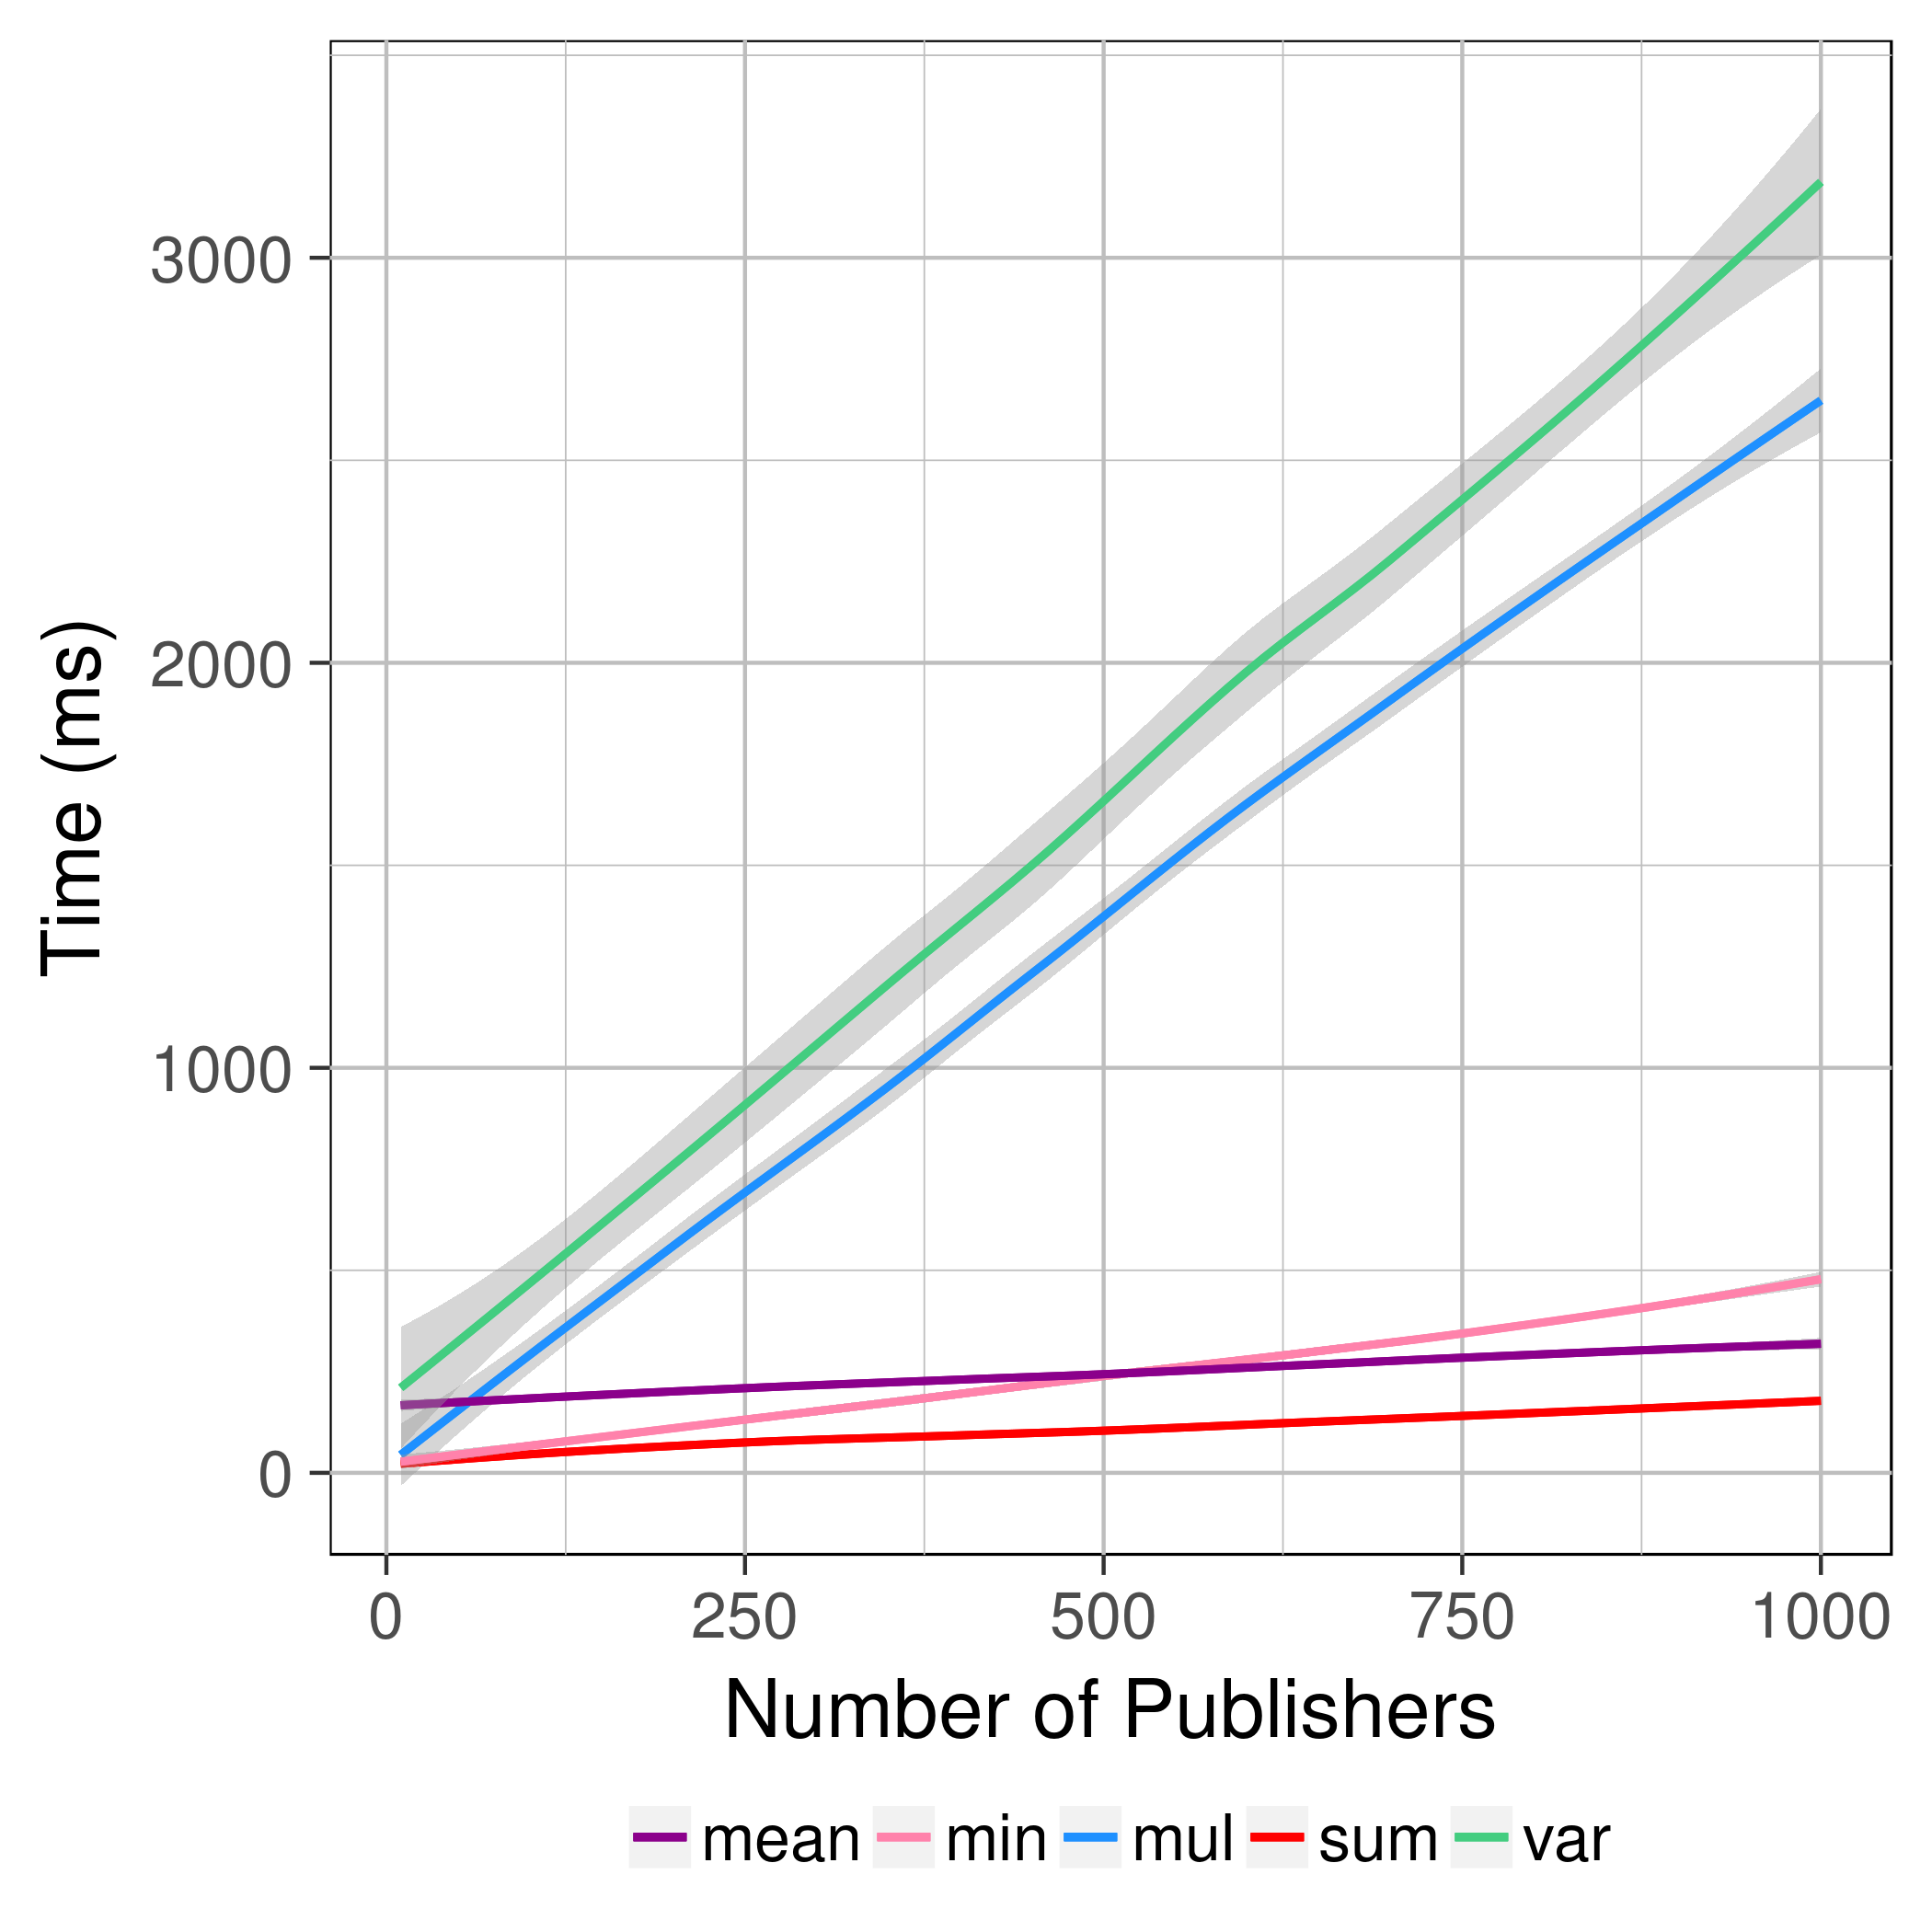
\includegraphics[width=\textwidth]{plots/send.png}
        \caption{Send}
        \label{fig:micro-send-time}
    \end{subfigure}
    \caption{Mean time required for garbling, evaluating and sending the
    garbled circuit to the Broker for each function in the microbenchmark, with
    a 95\% confidence intervals of the samples obtained in the evaluation shown
    in gray.  Sending includes the marshaling and unmarshaling of the garbled
    circuit and associated data structures.}\label{fig:micro-times}
\end{figure*}


\begin{figure}
  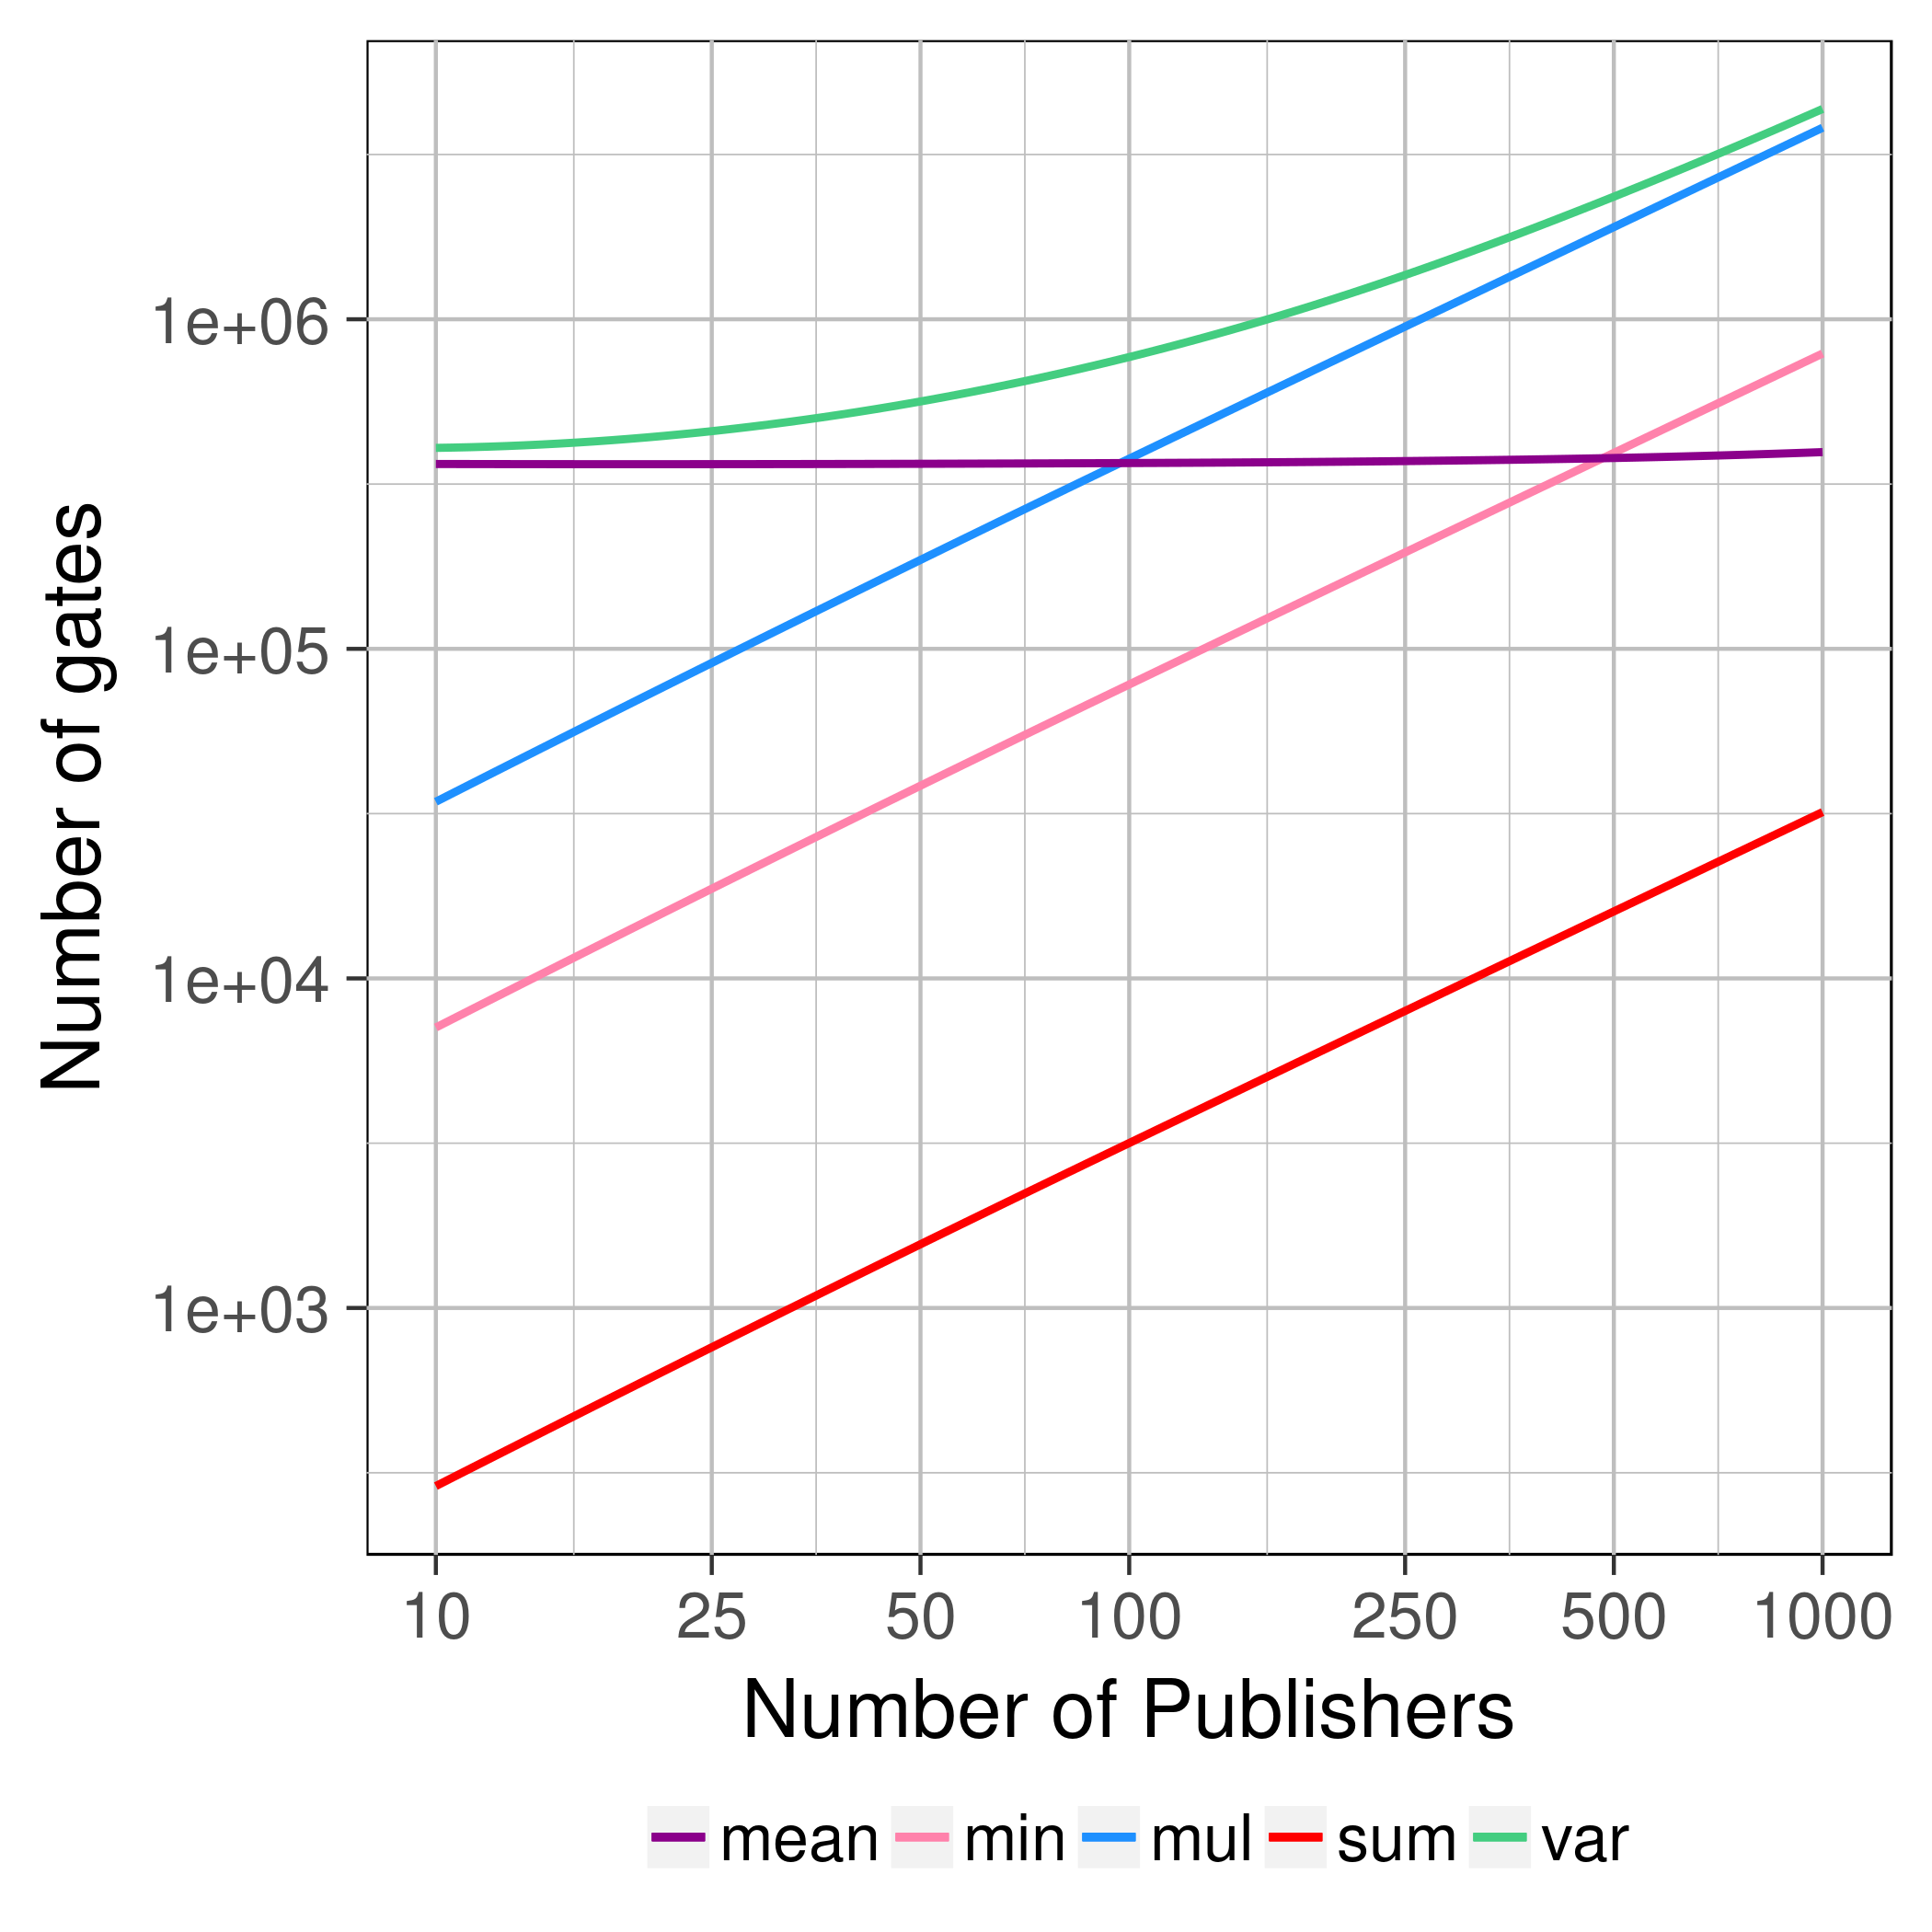
\includegraphics[width=0.45\textwidth]{plots/nonxor_gates_log.png}
  \caption{Gates count per function used in the microbenchmarks.}
  \label{micro-nonxor}
\end{figure}

\begin{figure}
  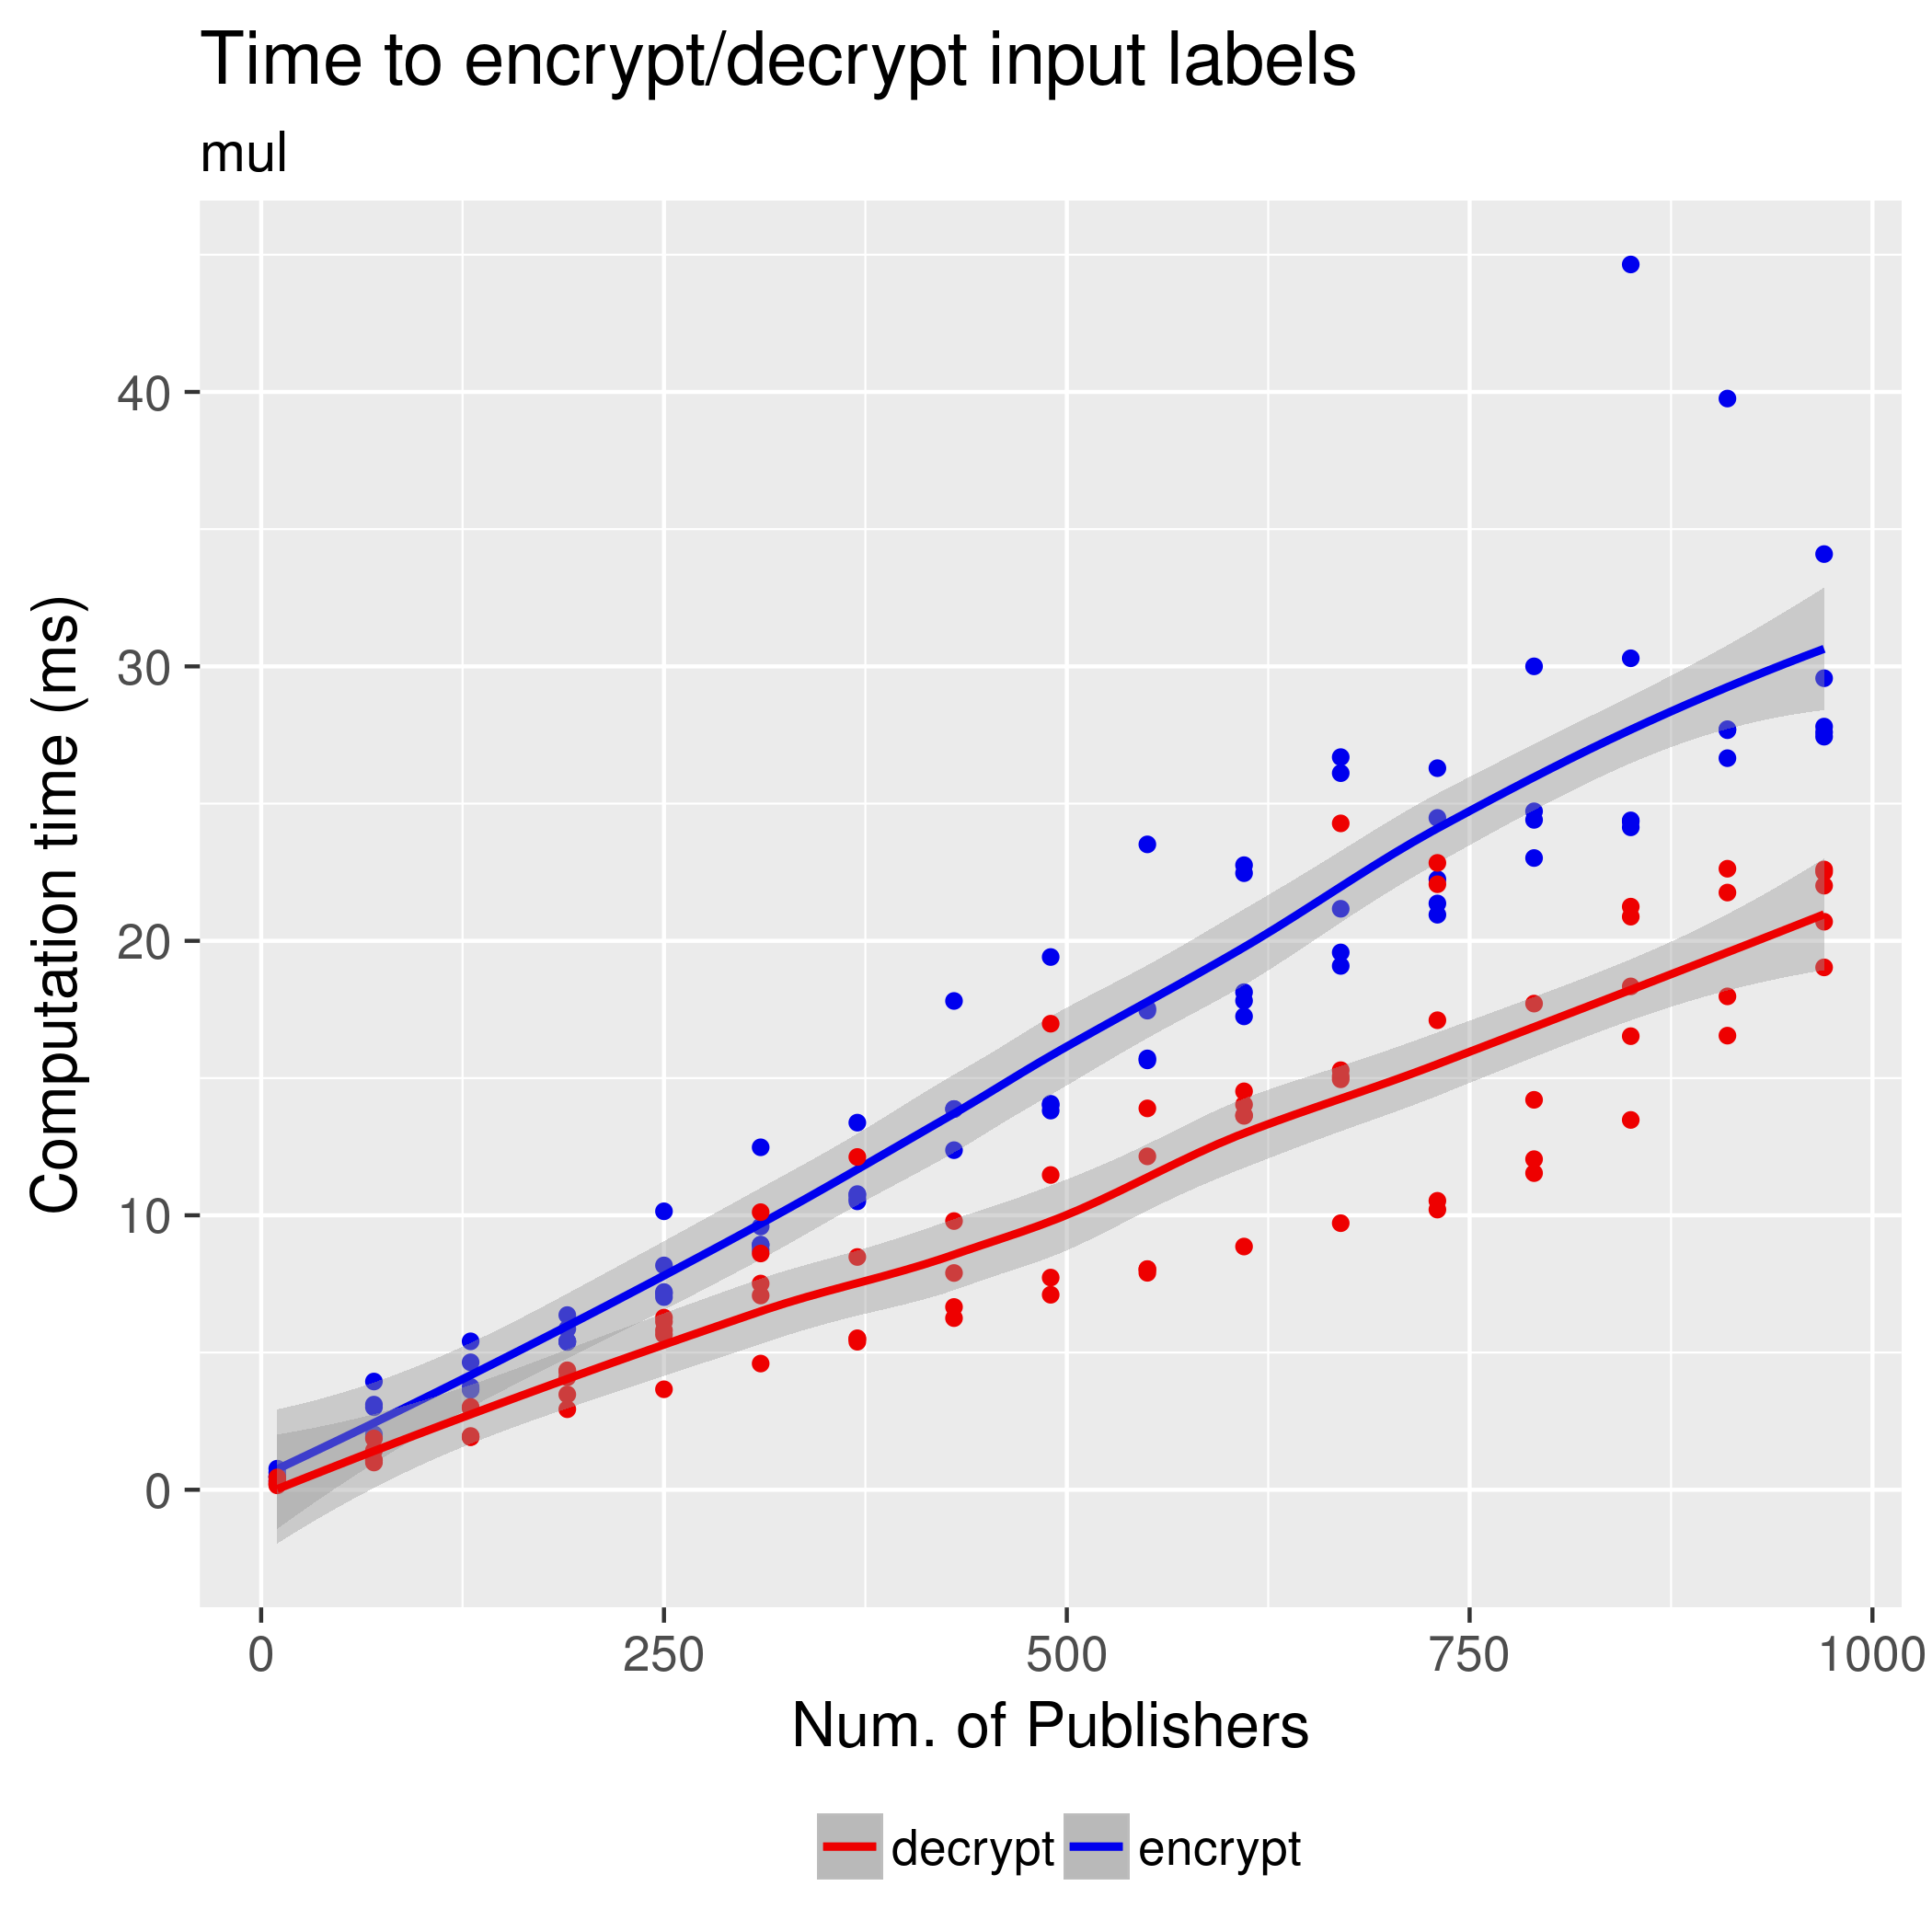
\includegraphics[width=0.45\textwidth]{plots/enc_dec_inputs.png}
  \caption{Time spent garbling and evaluating the identity input gates.}
  \label{micro-inputs}
\end{figure}

%\begin{figure}
%  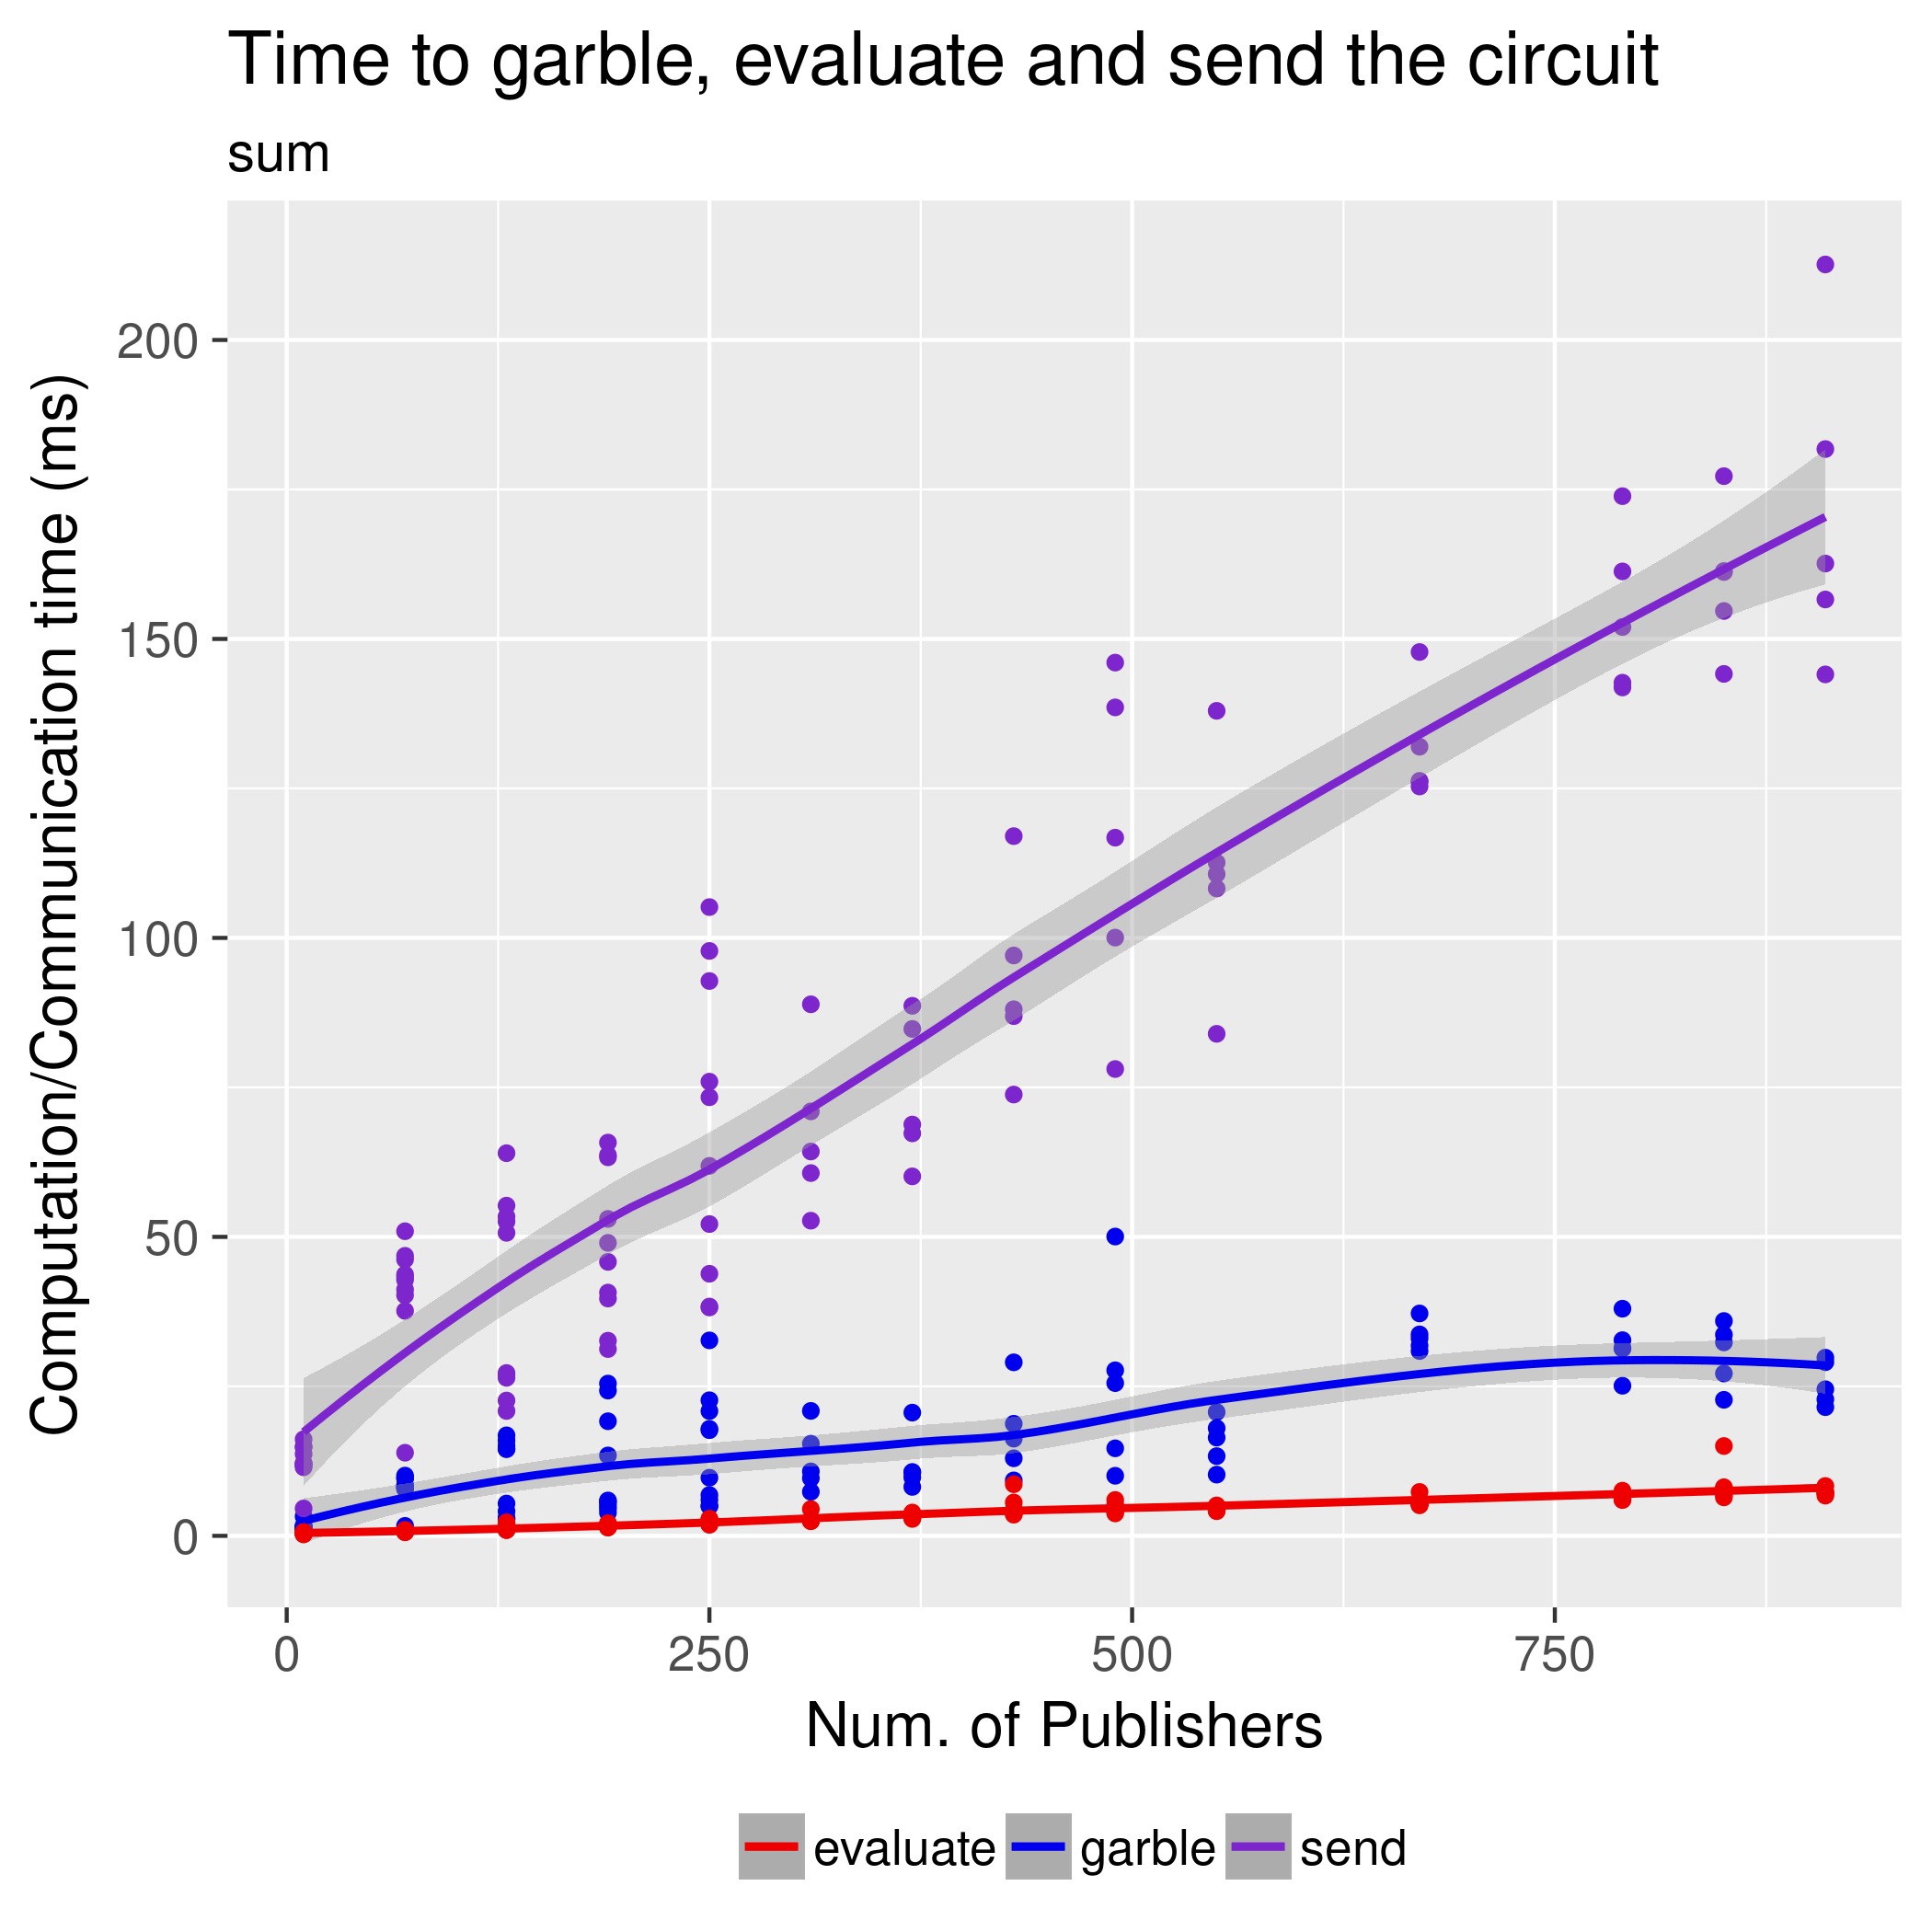
\includegraphics[width=0.45\textwidth]{plots/sum_circuit_2017-05-15.png}
%  \caption{Time spent garbling the circuit, sending the result to the Broker and evaluating it.}
%\end{figure}

%\begin{figure}
%  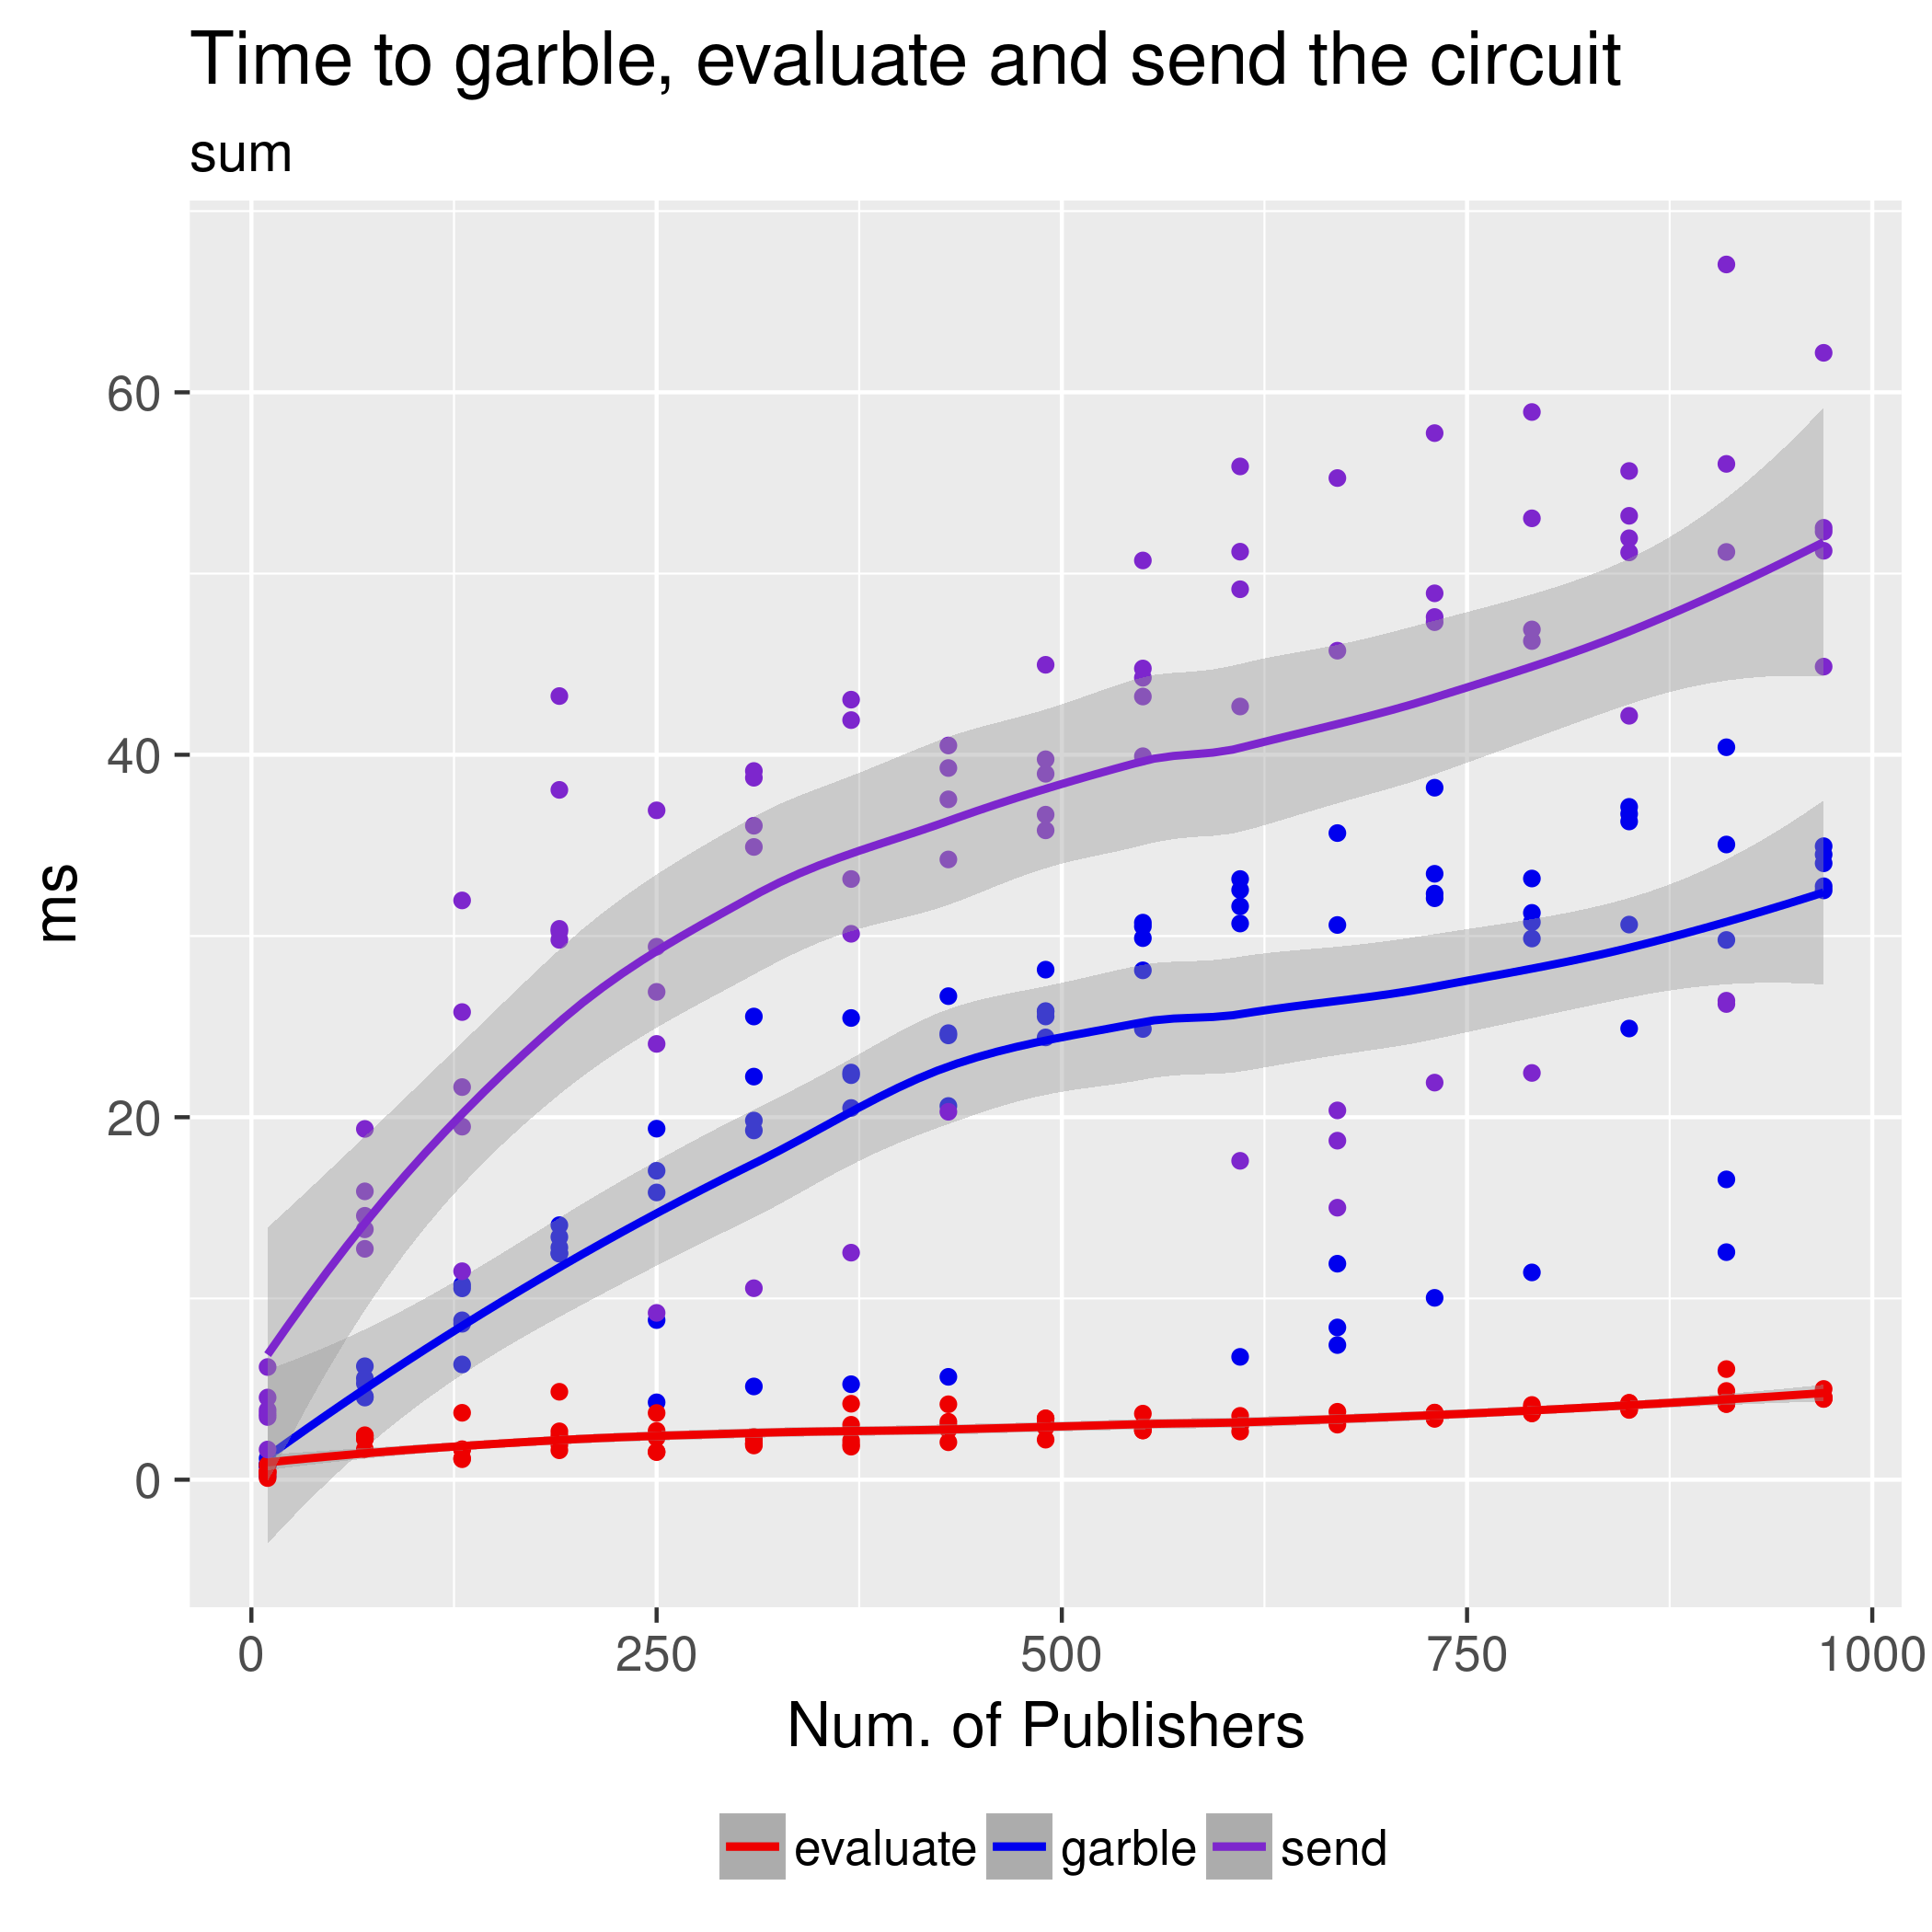
\includegraphics[width=0.45\textwidth]{plots/sum_circuit_onepub_2017-05-13.png}
%  \caption{Time spent garbling the circuit, sending the result to the Broker
%  and evaluating it removing the overhead of handling the Publishers
%  connections.}
%\end{figure}

\begin{figure}
  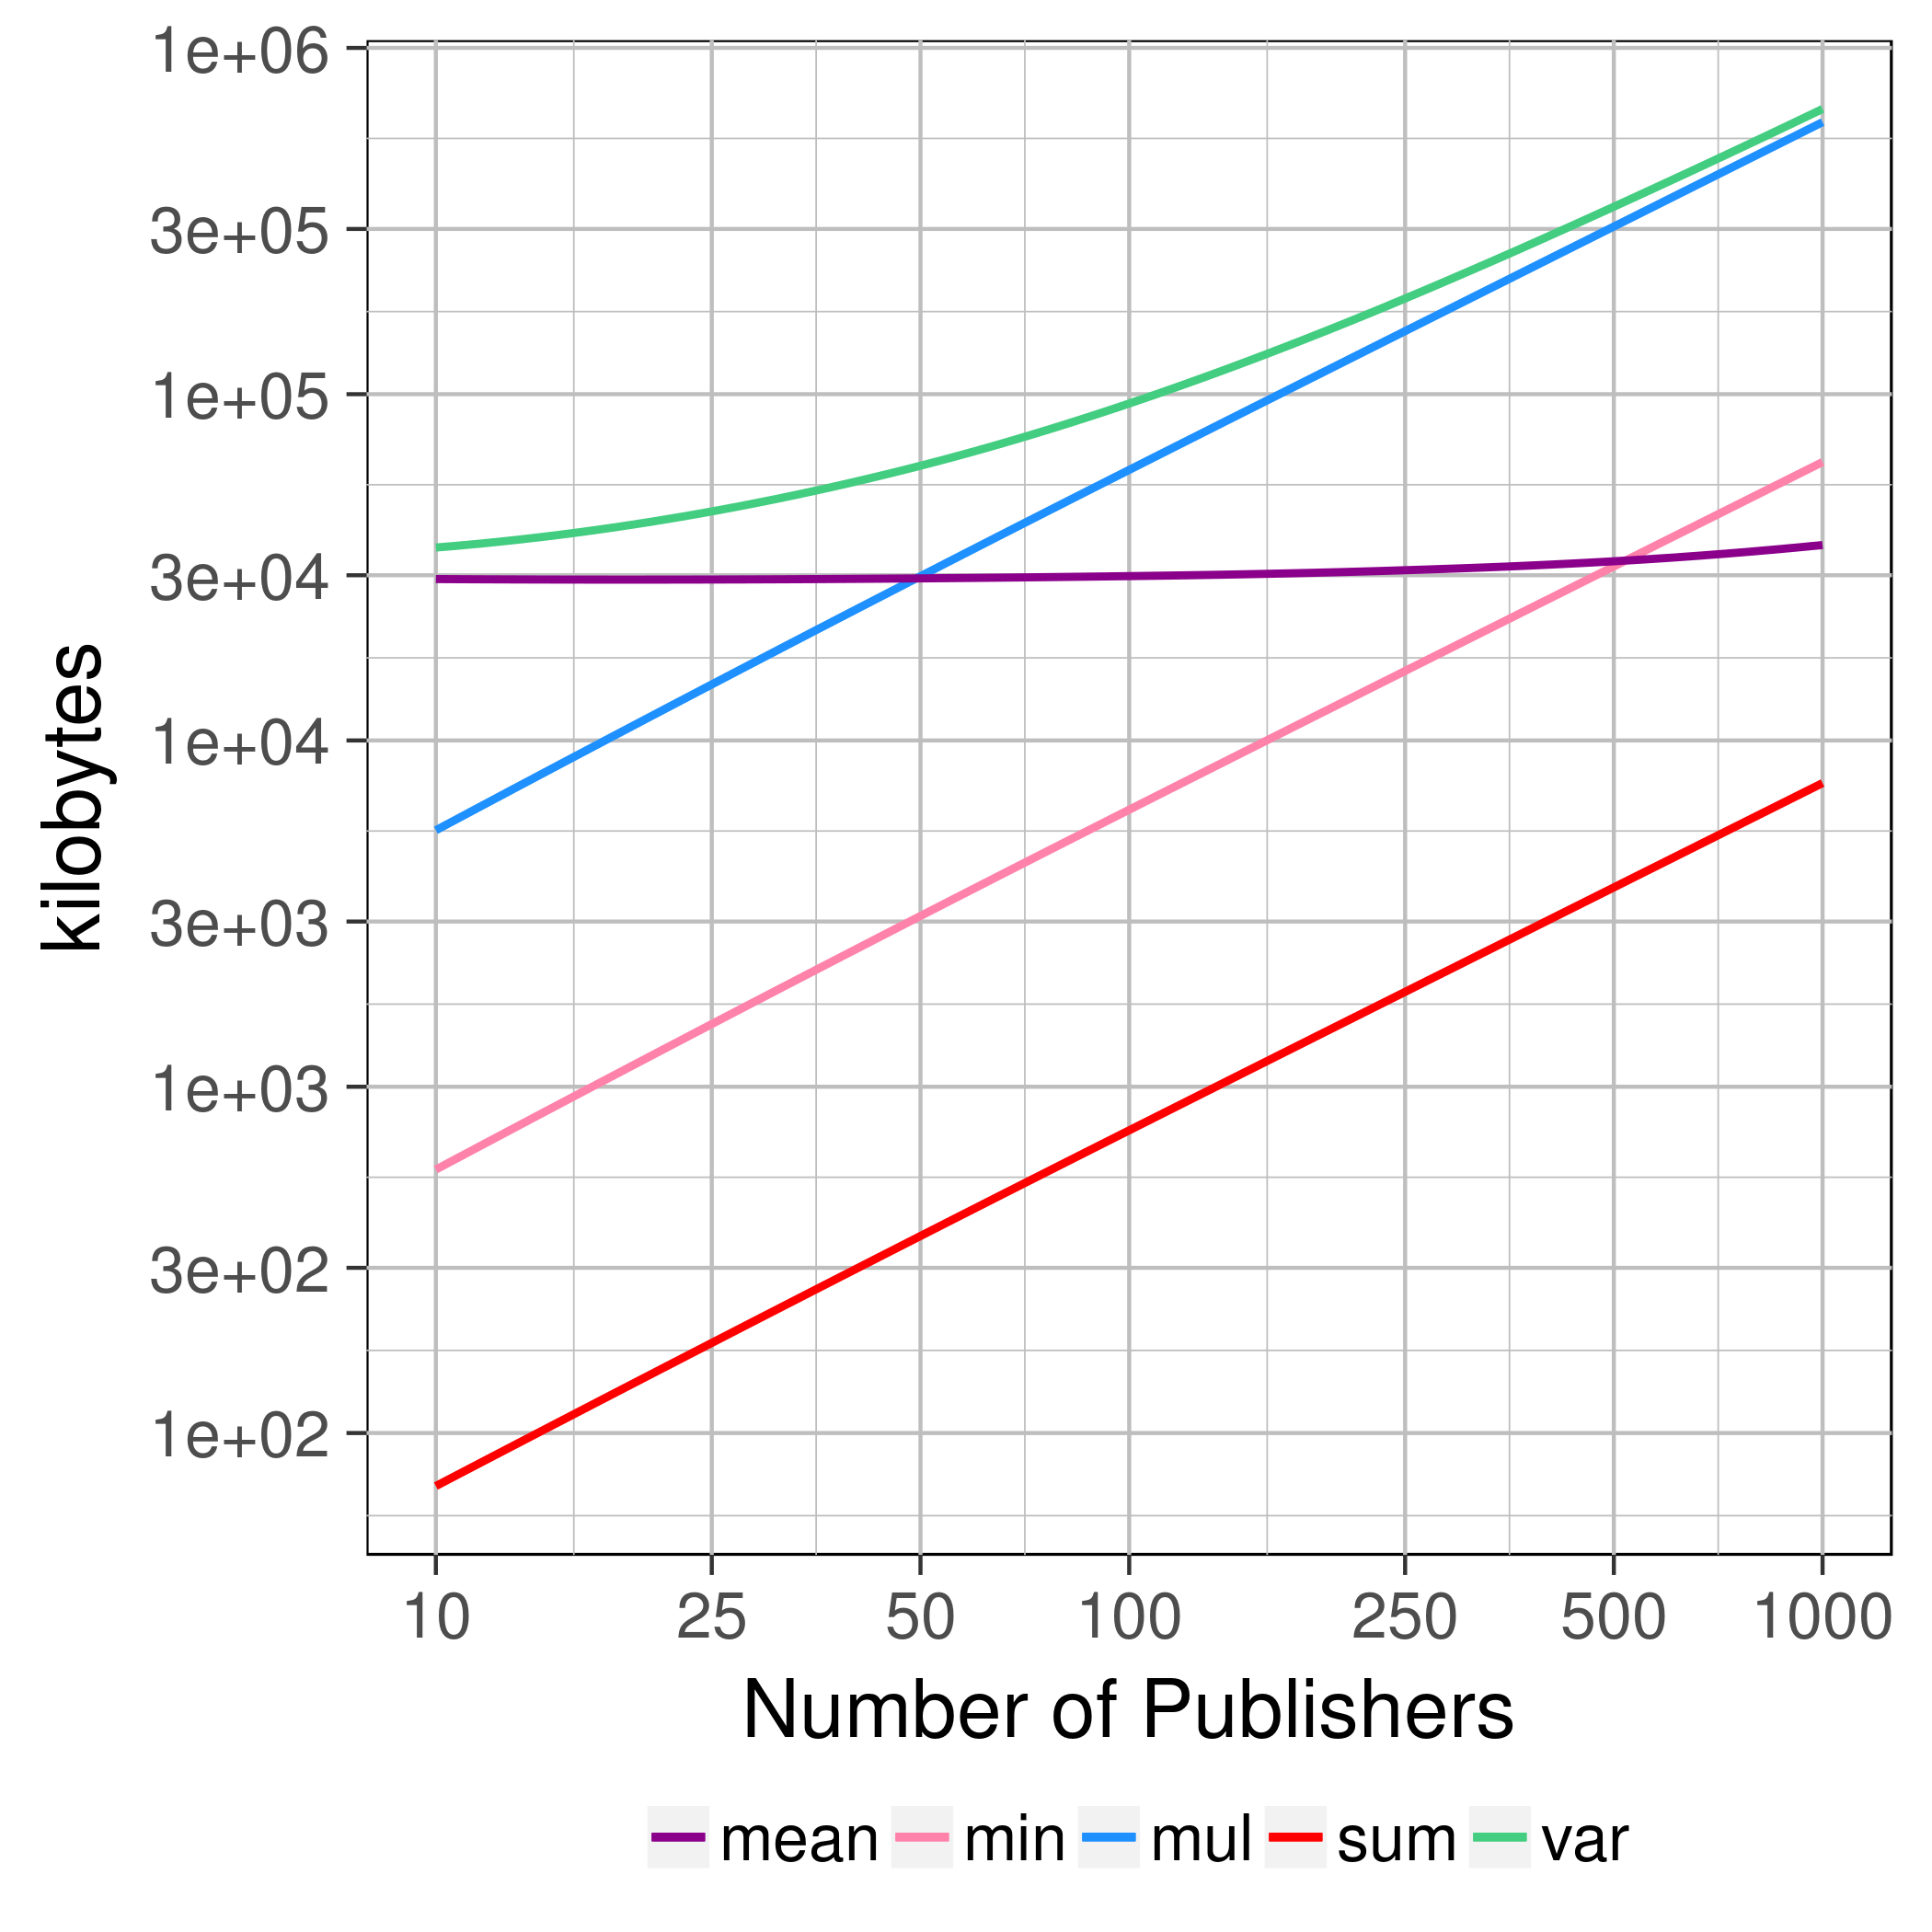
\includegraphics[width=0.45\textwidth]{plots/size_log.png}
  \caption{Size of the garbled circuit and the associated date required by the
  Broker to evaluate it.}
  \label{micro-sizes}
\end{figure}

We can see that the time spent encrypting and decrypting the inputs (that is,
garbling and evaluating the input identity gates) makes a significant influence
in the mean, min/max and sum microbenchmark, being comparable in magnitude to
the evaluation and garbling time (notice that for sum, the input
encryption/decryption time is even higher than the garbling/evaluation time).
We attribute this behavior to the fact that this part of the protocol is
implemented in go instead of C like the garbling and evaluation.

\subsection{Applications}

% TODO: 1. Environmental Berkeley indor sensing data, correlation
\paragraph{Correlation of two data streams}

% Questions: How many data points to use?

% Formula:

% We compute the correlation squared to avoid computing the square root in the
% function circuit, which would be an expensive operation.

% TODO: 2. Road Volume sensor traffic, evaluation of the expected time to follow a path
\paragraph{Estimation of time required to follow a path with traffic}

% http://rtmap.metro.net/ <- Not working (2017-05-15).

\begin{figure}
  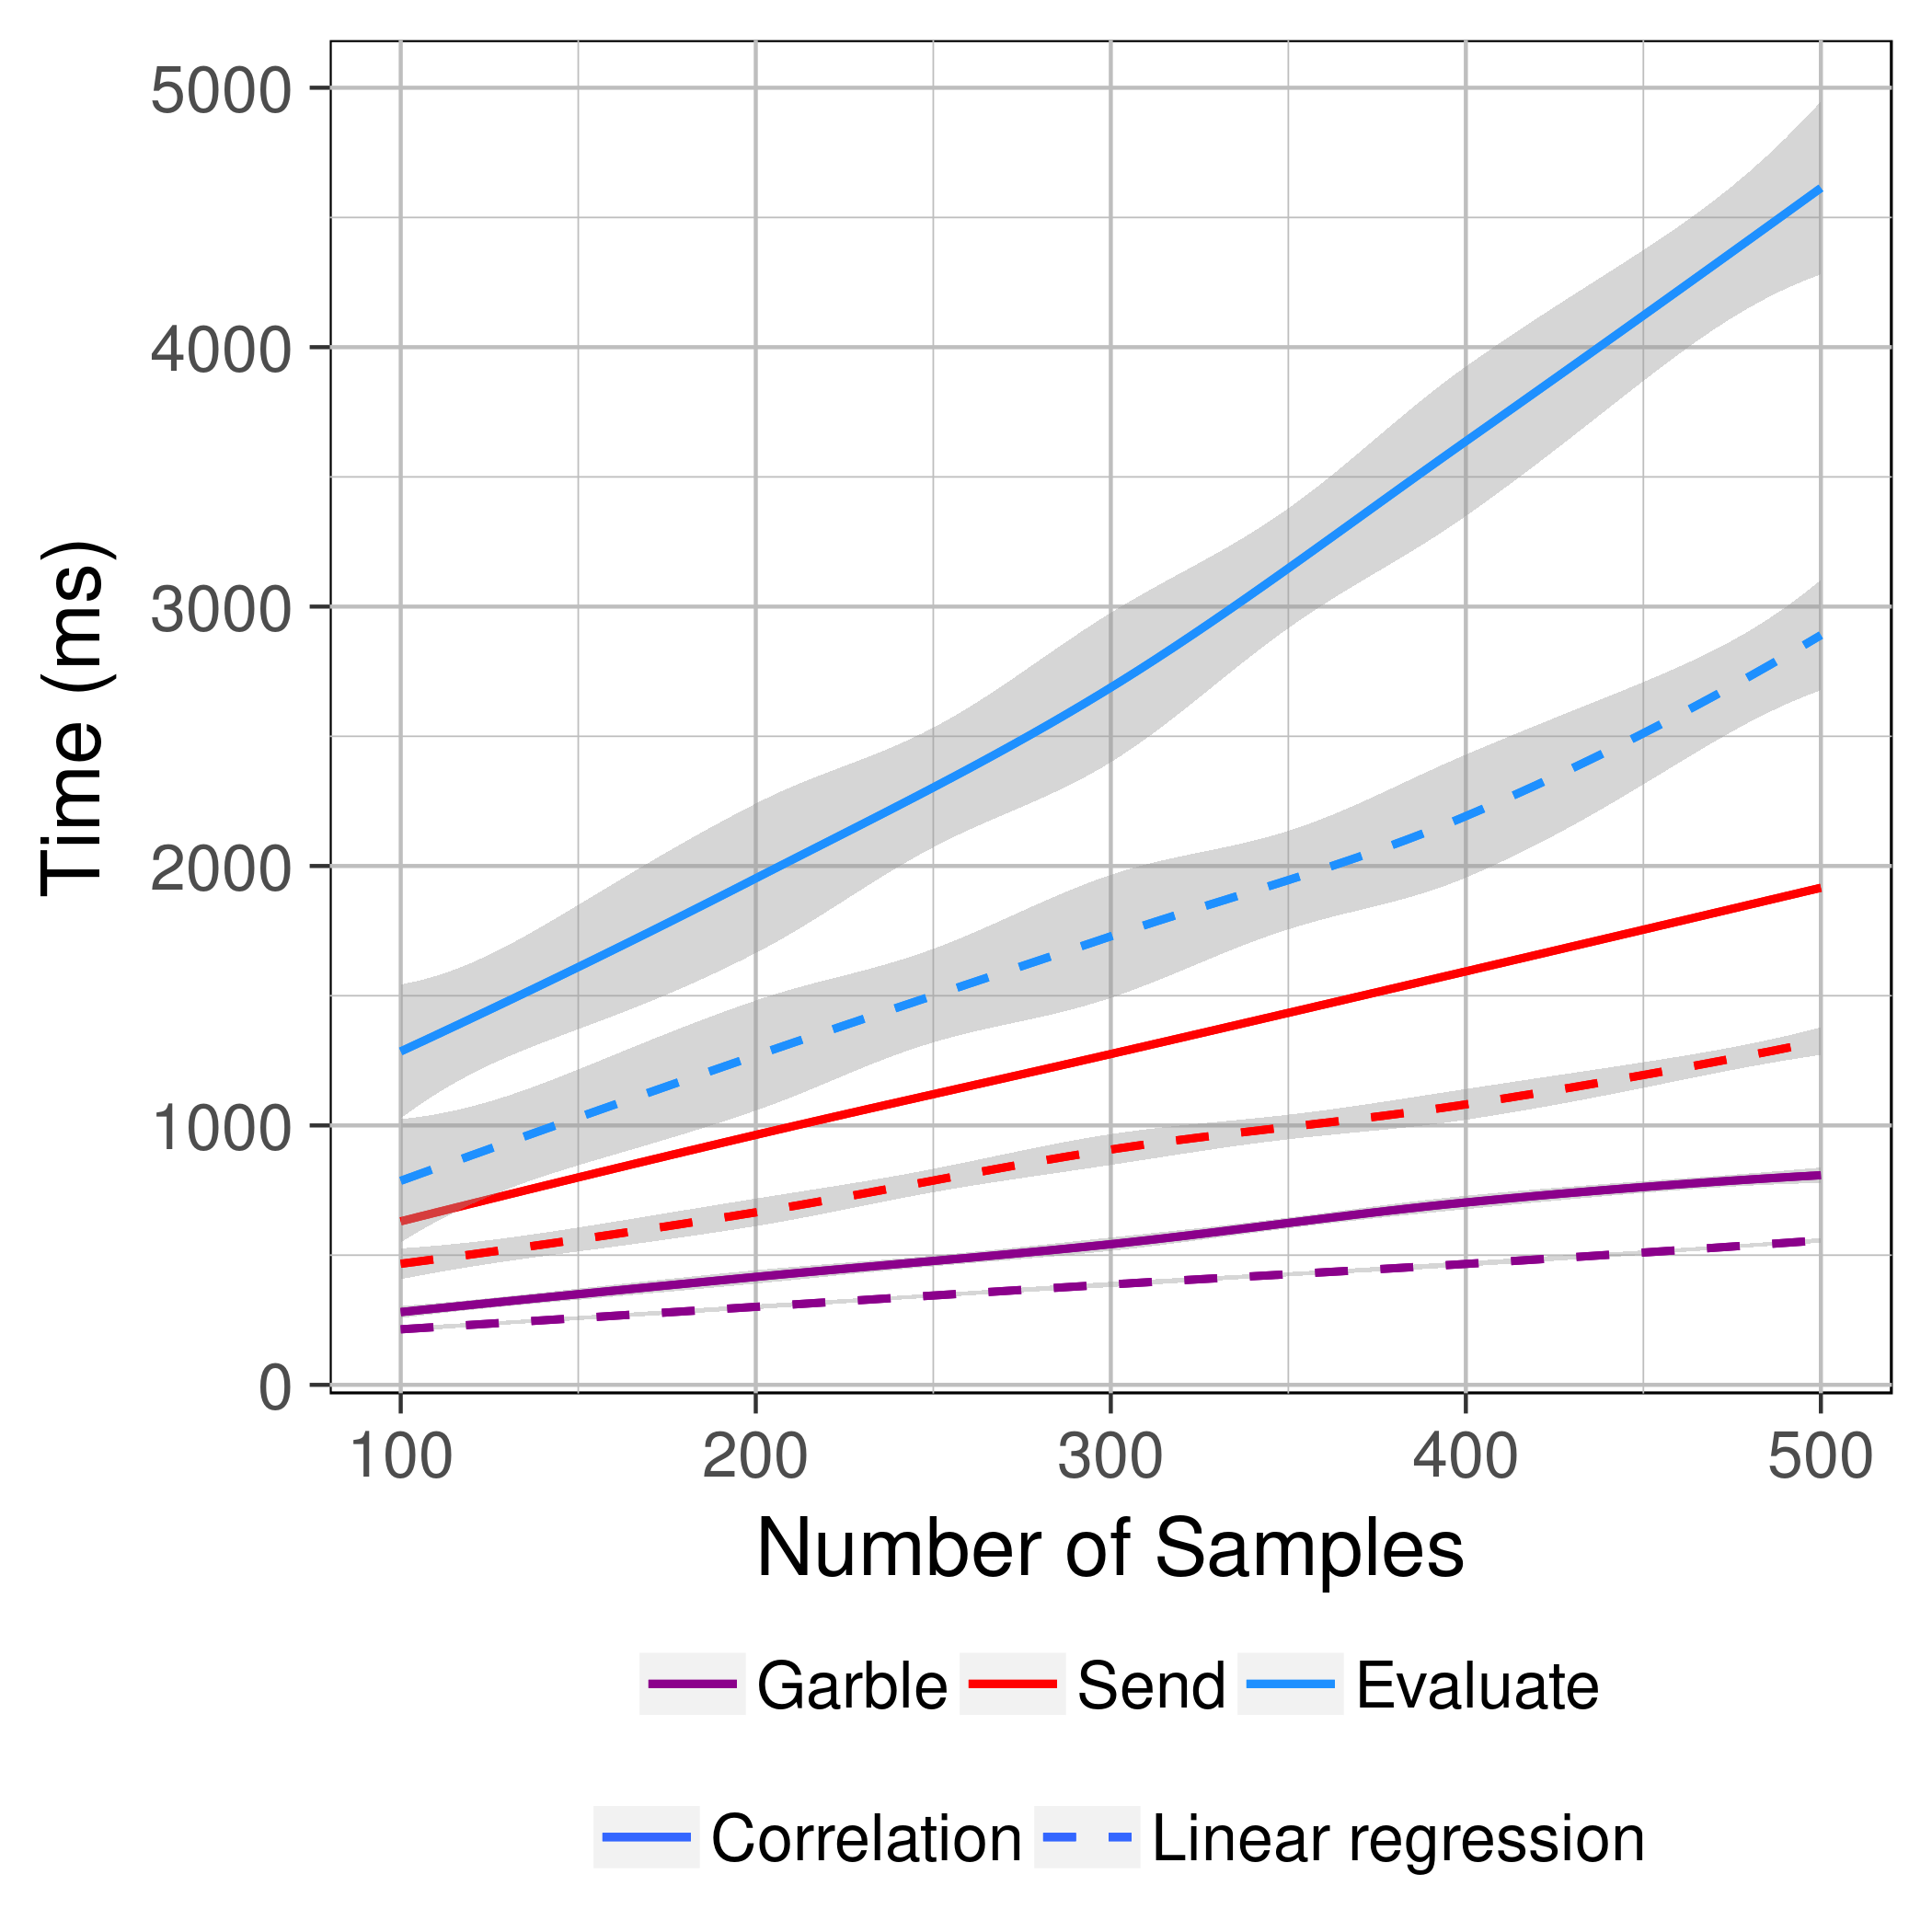
\includegraphics[width=0.45\textwidth]{plots/stream.png}
  \caption{Mean time required for garbling, evaluating and sending the garbled
  circuit to the Broker for computing the correlation and linear regression of
  data streams, with a 95\% confidence intervals of the samples obtained in the
  evaluation shown in gray.  Sending includes the marshaling and unmarshaling
  of the garbled circuit and associated data structures.  Garbling and
  evaluating includes the time to garble and evaluate the input identity.}
  \label{stream-times}
\end{figure}

% TODO: 3. LAX parking lot dataset, statistics
\paragraph{Continuous statistics of incoming data}

% https://data.lacity.org/dataset/Los-Angeles-International-Airport-LAX-Parking-Lots/dik5-hwp6
% The dataset provides at a frequency of every 5 minutes and for every one of
% the 9 parking lots: total, occupied and free parking spaces.
% That's 288 values per day per parking lot.

% Privacy: Avoid revealing parking lot data at fine granularity, only reveal
% statistics of the data accumulated throughout the day.  Don't reveal data of
% individual parking lots, only combined data (except for the lot with
% more/less free spots)

% Setting: We have 9 Publishers, one for each lot, which send data (current
% number of free spots, current number of used spots) every 5 minutes.  The
% Broker accumulates the data of a day and computes the statistics.  This
% happens once per day.

% Daily statistics (used spots): mean, max, min, var of the number of cars in all the lots combined.
% Daily statistics (free spots): The marking lot which had more free spots, and the one
% that had less on average during the day.

% Time garble and time eval includes the time spend encrypting and decrypting
% the input values.

% "mean time_garble = 199.7968218 time_send = 226.0614956 time_eval = 98.731150 size = 46867188"
% "max  time_garble = 163.2894558 time_send = 172.3834538 time_eval = 84.937214 size = 33530724"
% "min  time_garble = 164.4096572 time_send = 165.7728326 time_eval = 84.142138 size = 33530724"
% "var  time_garble = 500.6605406 time_send = 1055.636931 time_eval = 236.08728 size = 232874164"

% "max_free time_garble = 121.2790726 time_send = 85.043922 time_eval = 67.5544586 size = 17469252"
% "min_free time_garble = 120.9805436 time_send = 85.586087 time_eval = 67.8169886 size = 17469252"

% TODO: 4. Turonet, wireless propagation constant, linear regression
\paragraph{One dimensional linear regression}

% The dataset provides 2.3 million readings collected from sensors with the
% following values: temperature (degree Celcius), humidity (0-100%), light
% (Lux: 0-100000), identified by sensor ID.

% Ideas: correlation temperature~humidity, temperature~light.
% Questions: How many data points to use?
% Graph: varying number of points, do sampling

% Formula:

% TODO: 5. Smart bill, monthly electricity bill with different cost per hour of the day / threshold.

% ???

% Plots

% TODO: Discussion: bottlenecks.
% Sending the garbled circuit.
